\newpage
\appendix
\chapter{List of all categories and initial codes}

Appendix A contains a list of all the categories and initial codes used in this research project. Initial codes appear within the category that subsumed them. Initial codes were used to in the line-by-line coding for the first five articles analysed. Thereafter, categories were used to code the remaining articles. Coded references related to initial codes then referred to the category they belonged to.

\begin{landscape}
\begin{table}[h]
\centering
\bigskip\bigskip\bigskip
\caption{List of all categories and initial codes}
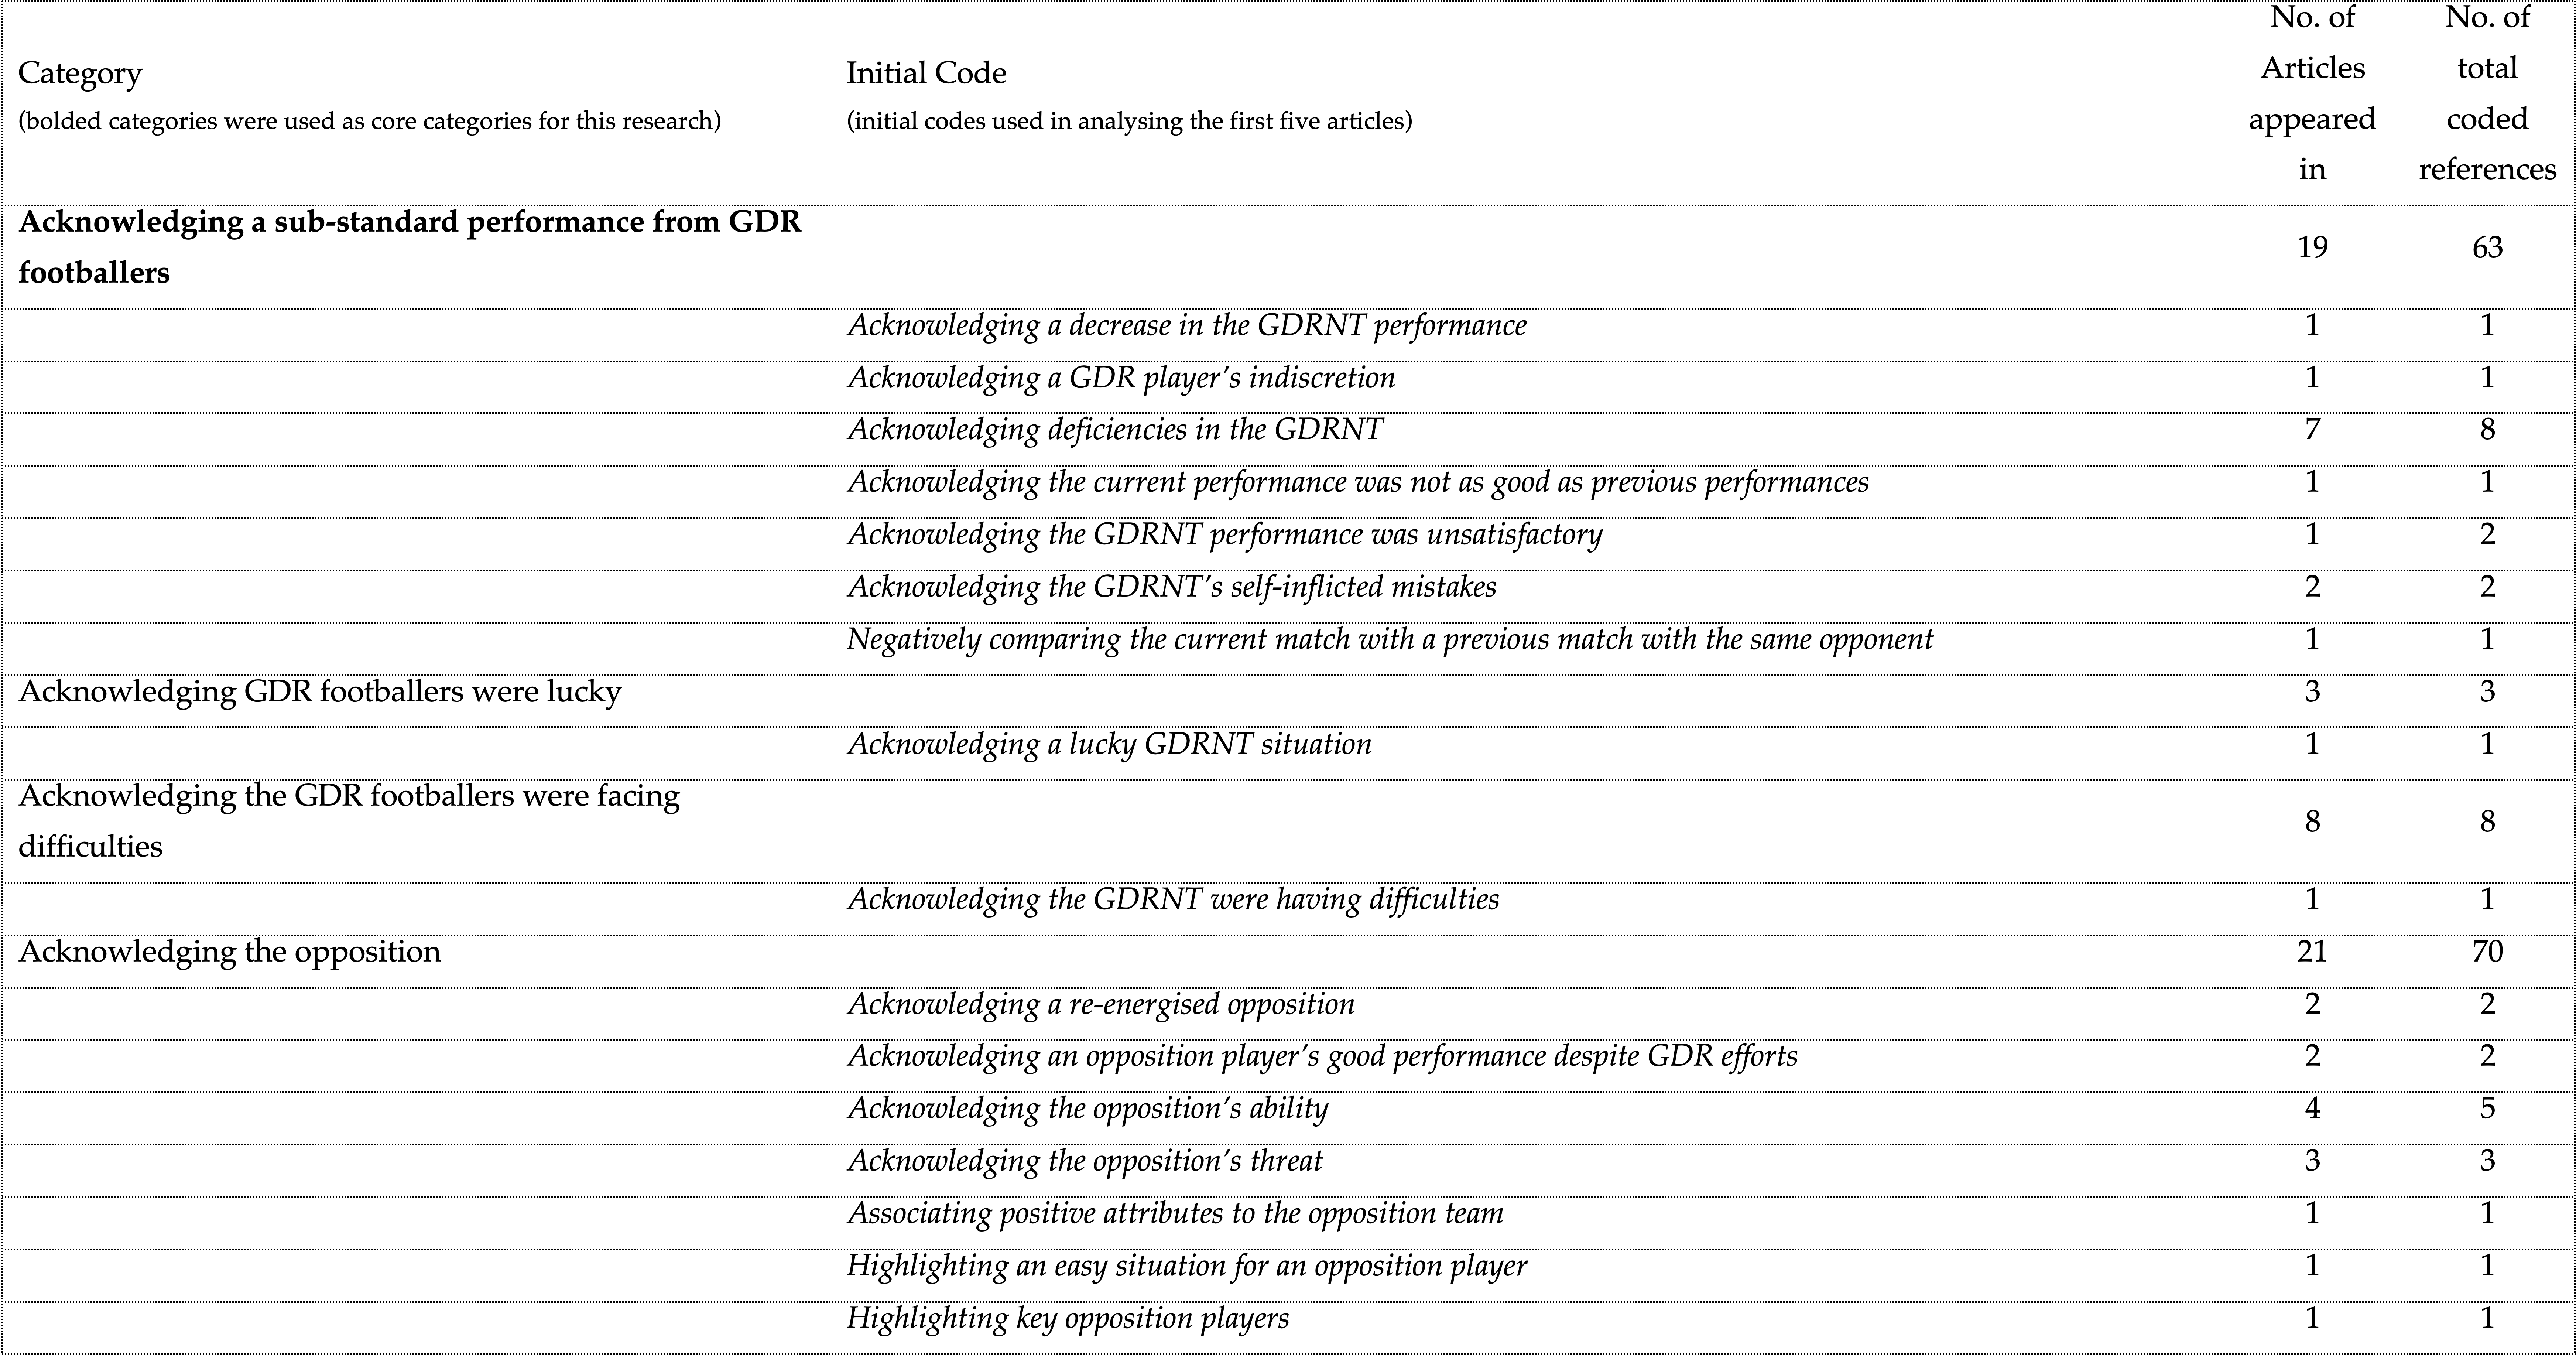
\includegraphics[width=\linewidth]{mres/images/appendix/a1.png}
\end{table}
\end{landscape}

\begin{landscape}
\begin{figure}[h]
\centering
\bigskip\bigskip\bigskip\bigskip\bigskip
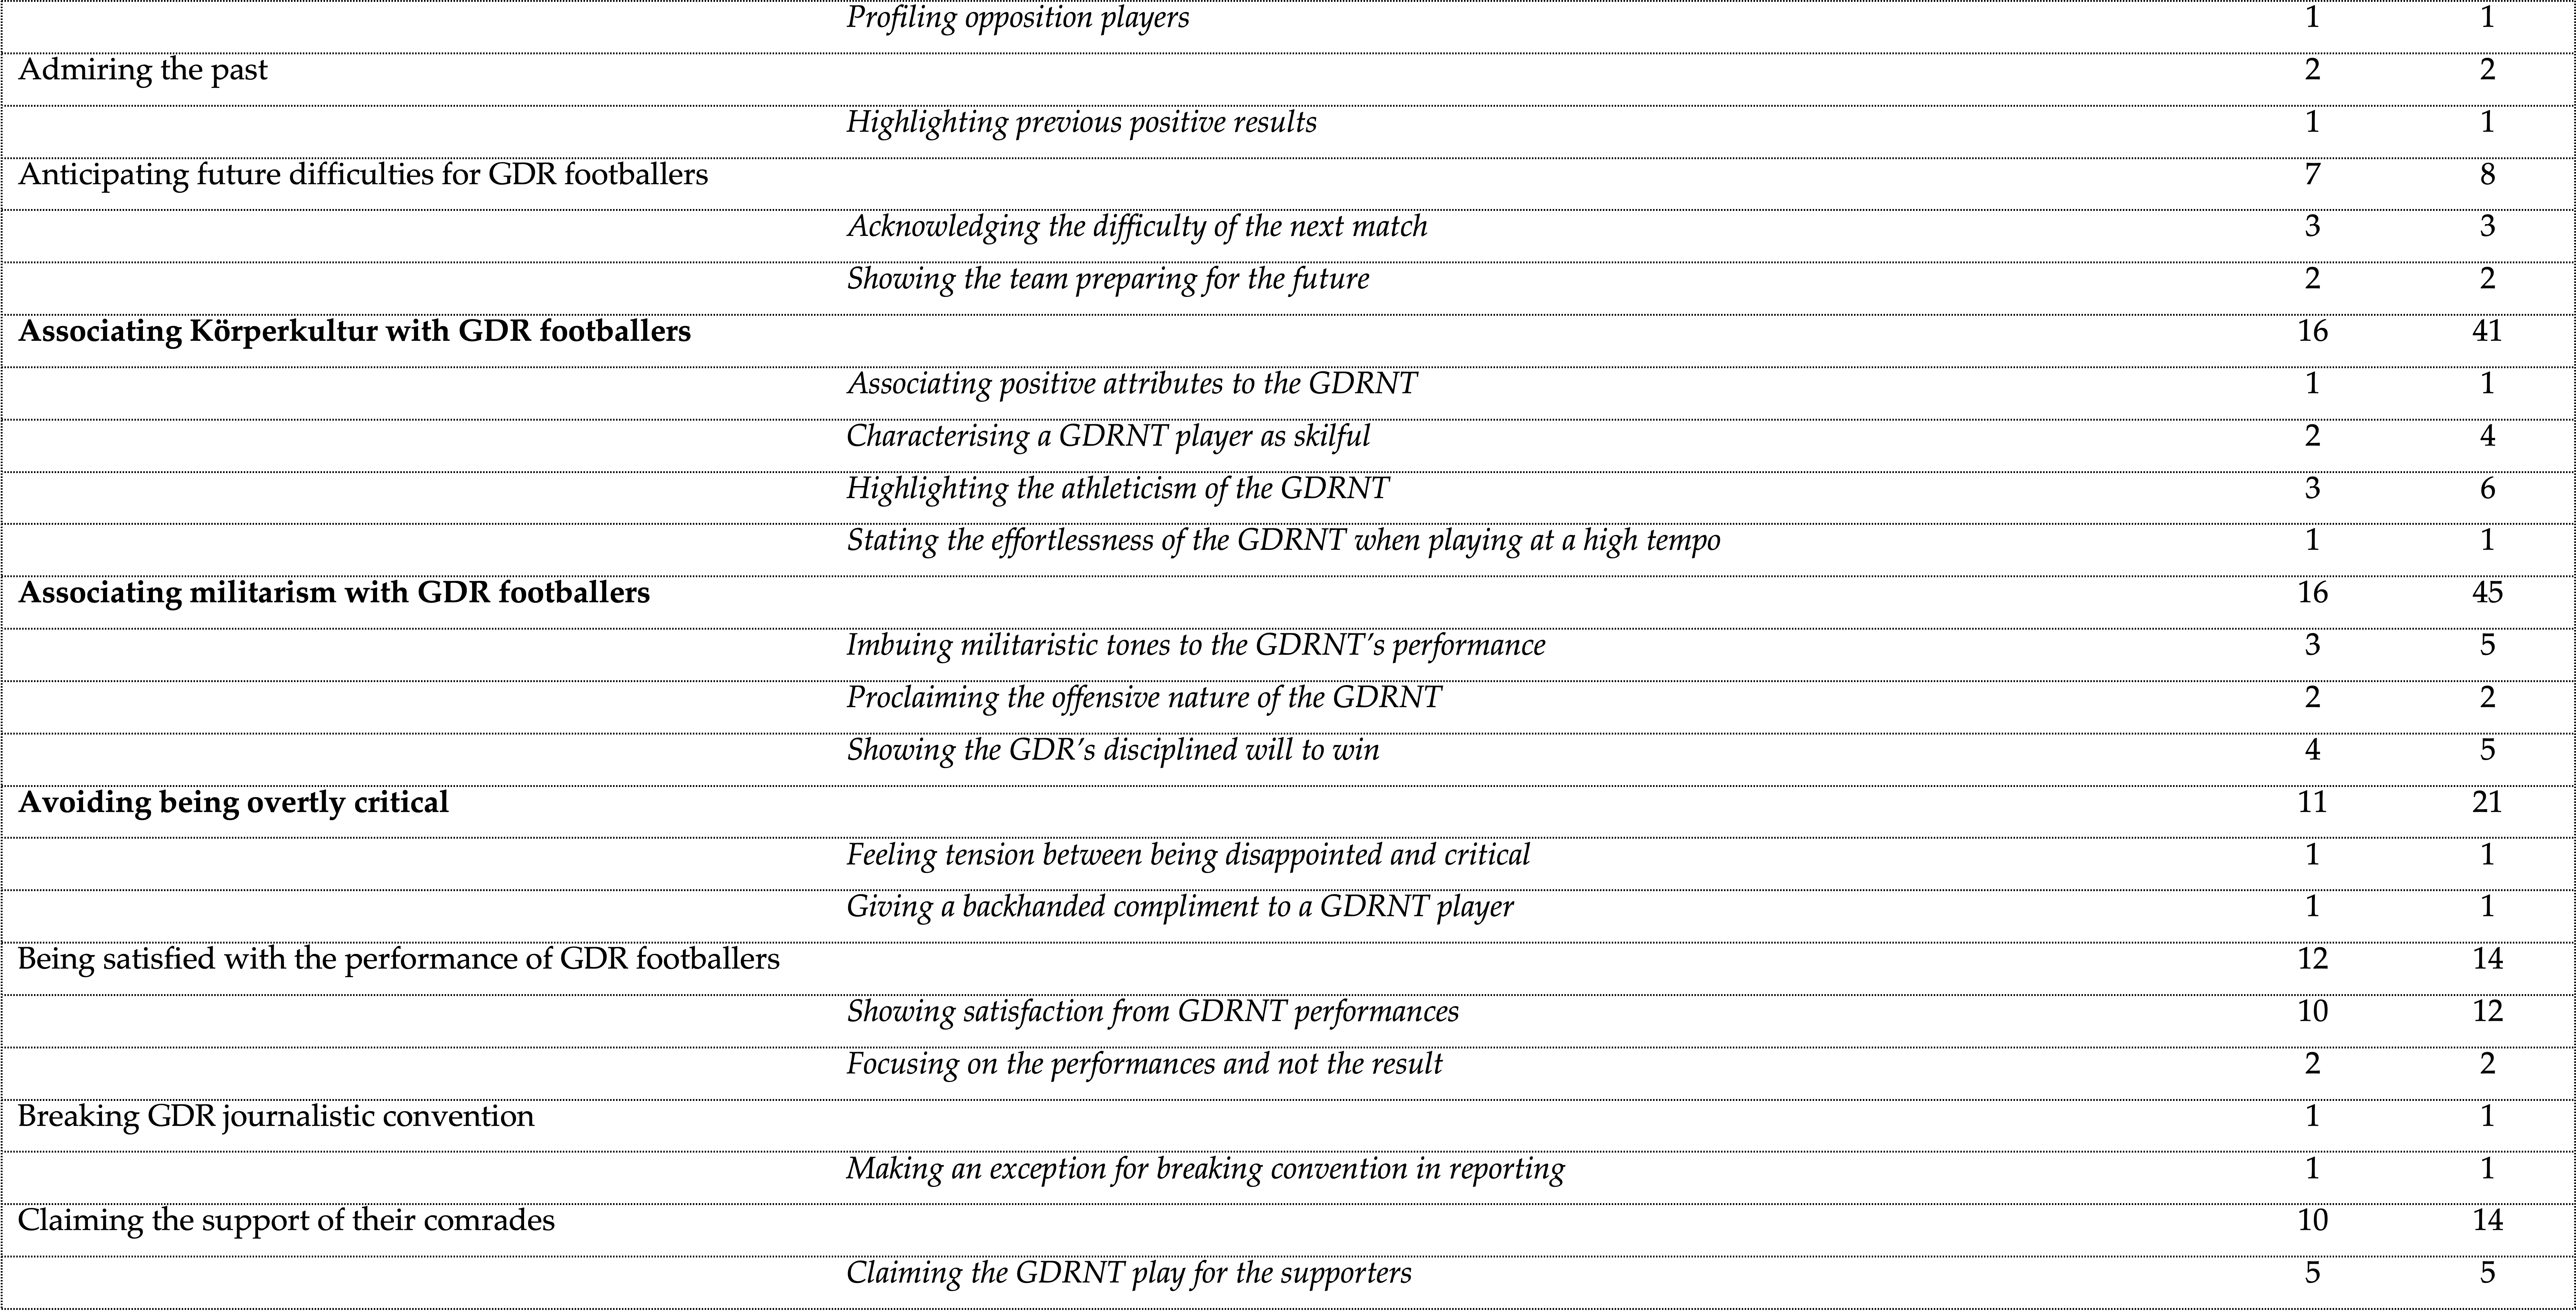
\includegraphics[width=\linewidth]{mres/images/appendix/a2.png}
\end{figure}
\end{landscape}

\begin{landscape}
\begin{figure}[h]
\centering
\bigskip\bigskip\bigskip\bigskip\bigskip
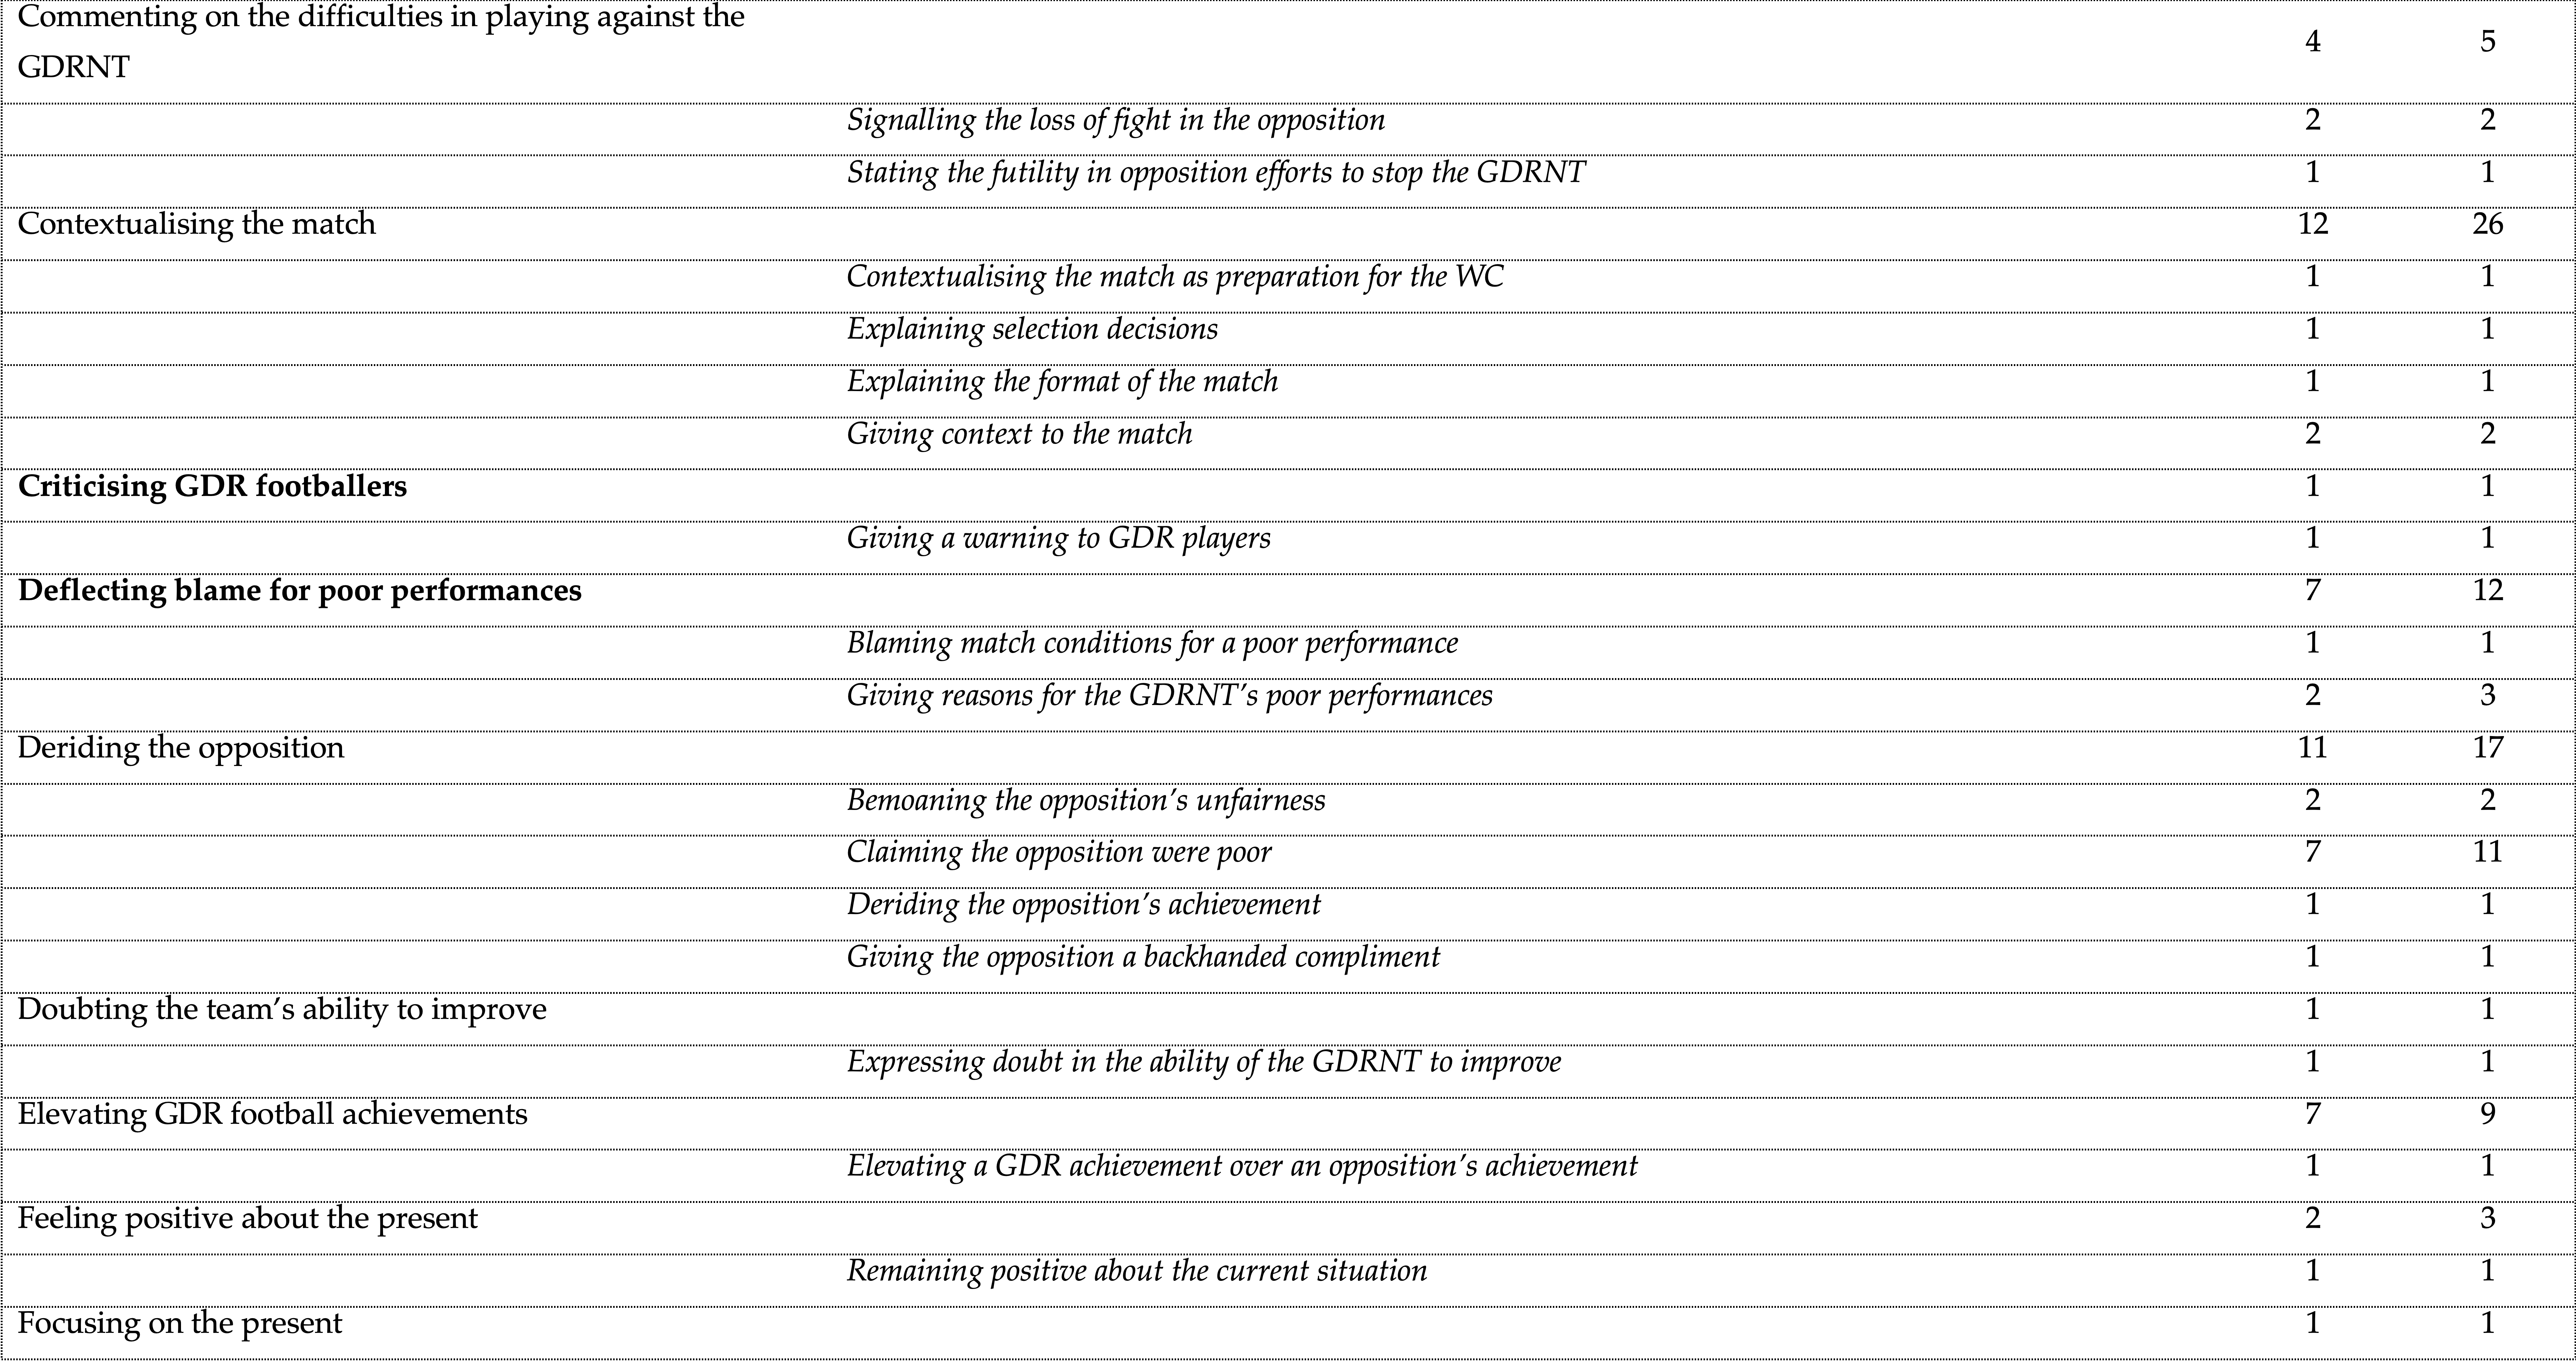
\includegraphics[width=\linewidth]{mres/images/appendix/a3.png}
\end{figure}
\end{landscape}

\begin{landscape}
\begin{figure}[h]
\centering
\bigskip\bigskip\bigskip\bigskip\bigskip
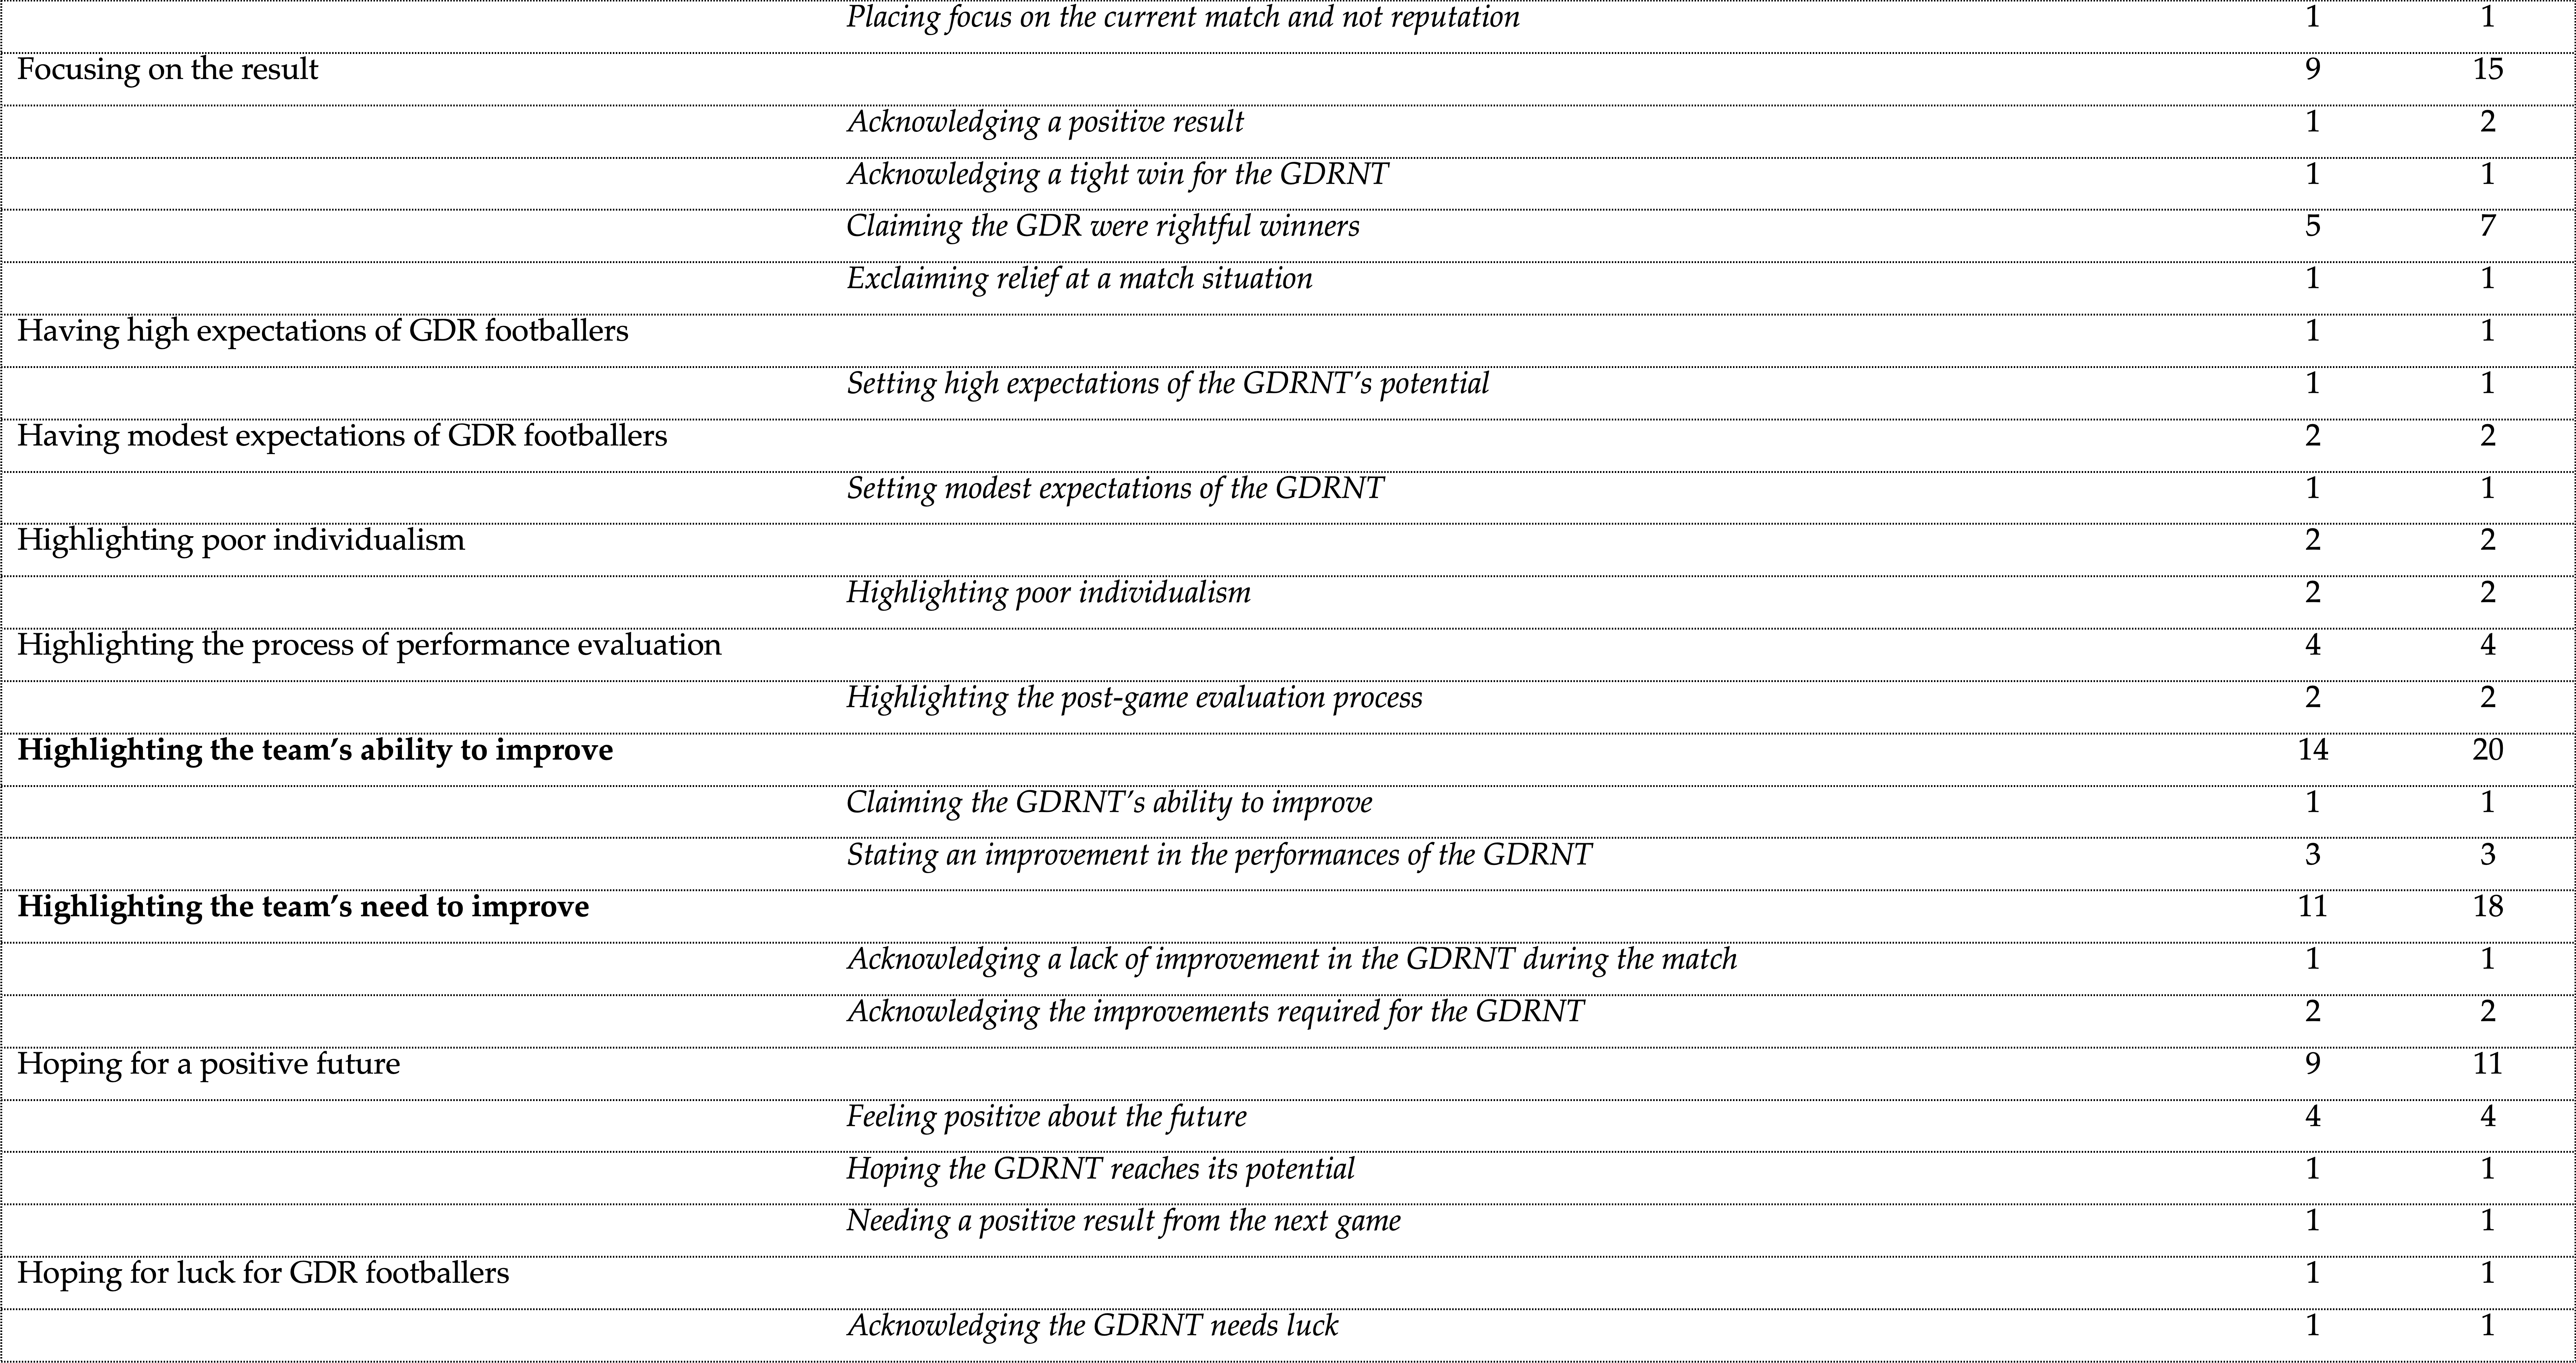
\includegraphics[width=\linewidth]{mres/images/appendix/a4.png}
\end{figure}
\end{landscape}

\begin{landscape}
\begin{figure}[h]
\centering
\bigskip\bigskip\bigskip\bigskip\bigskip
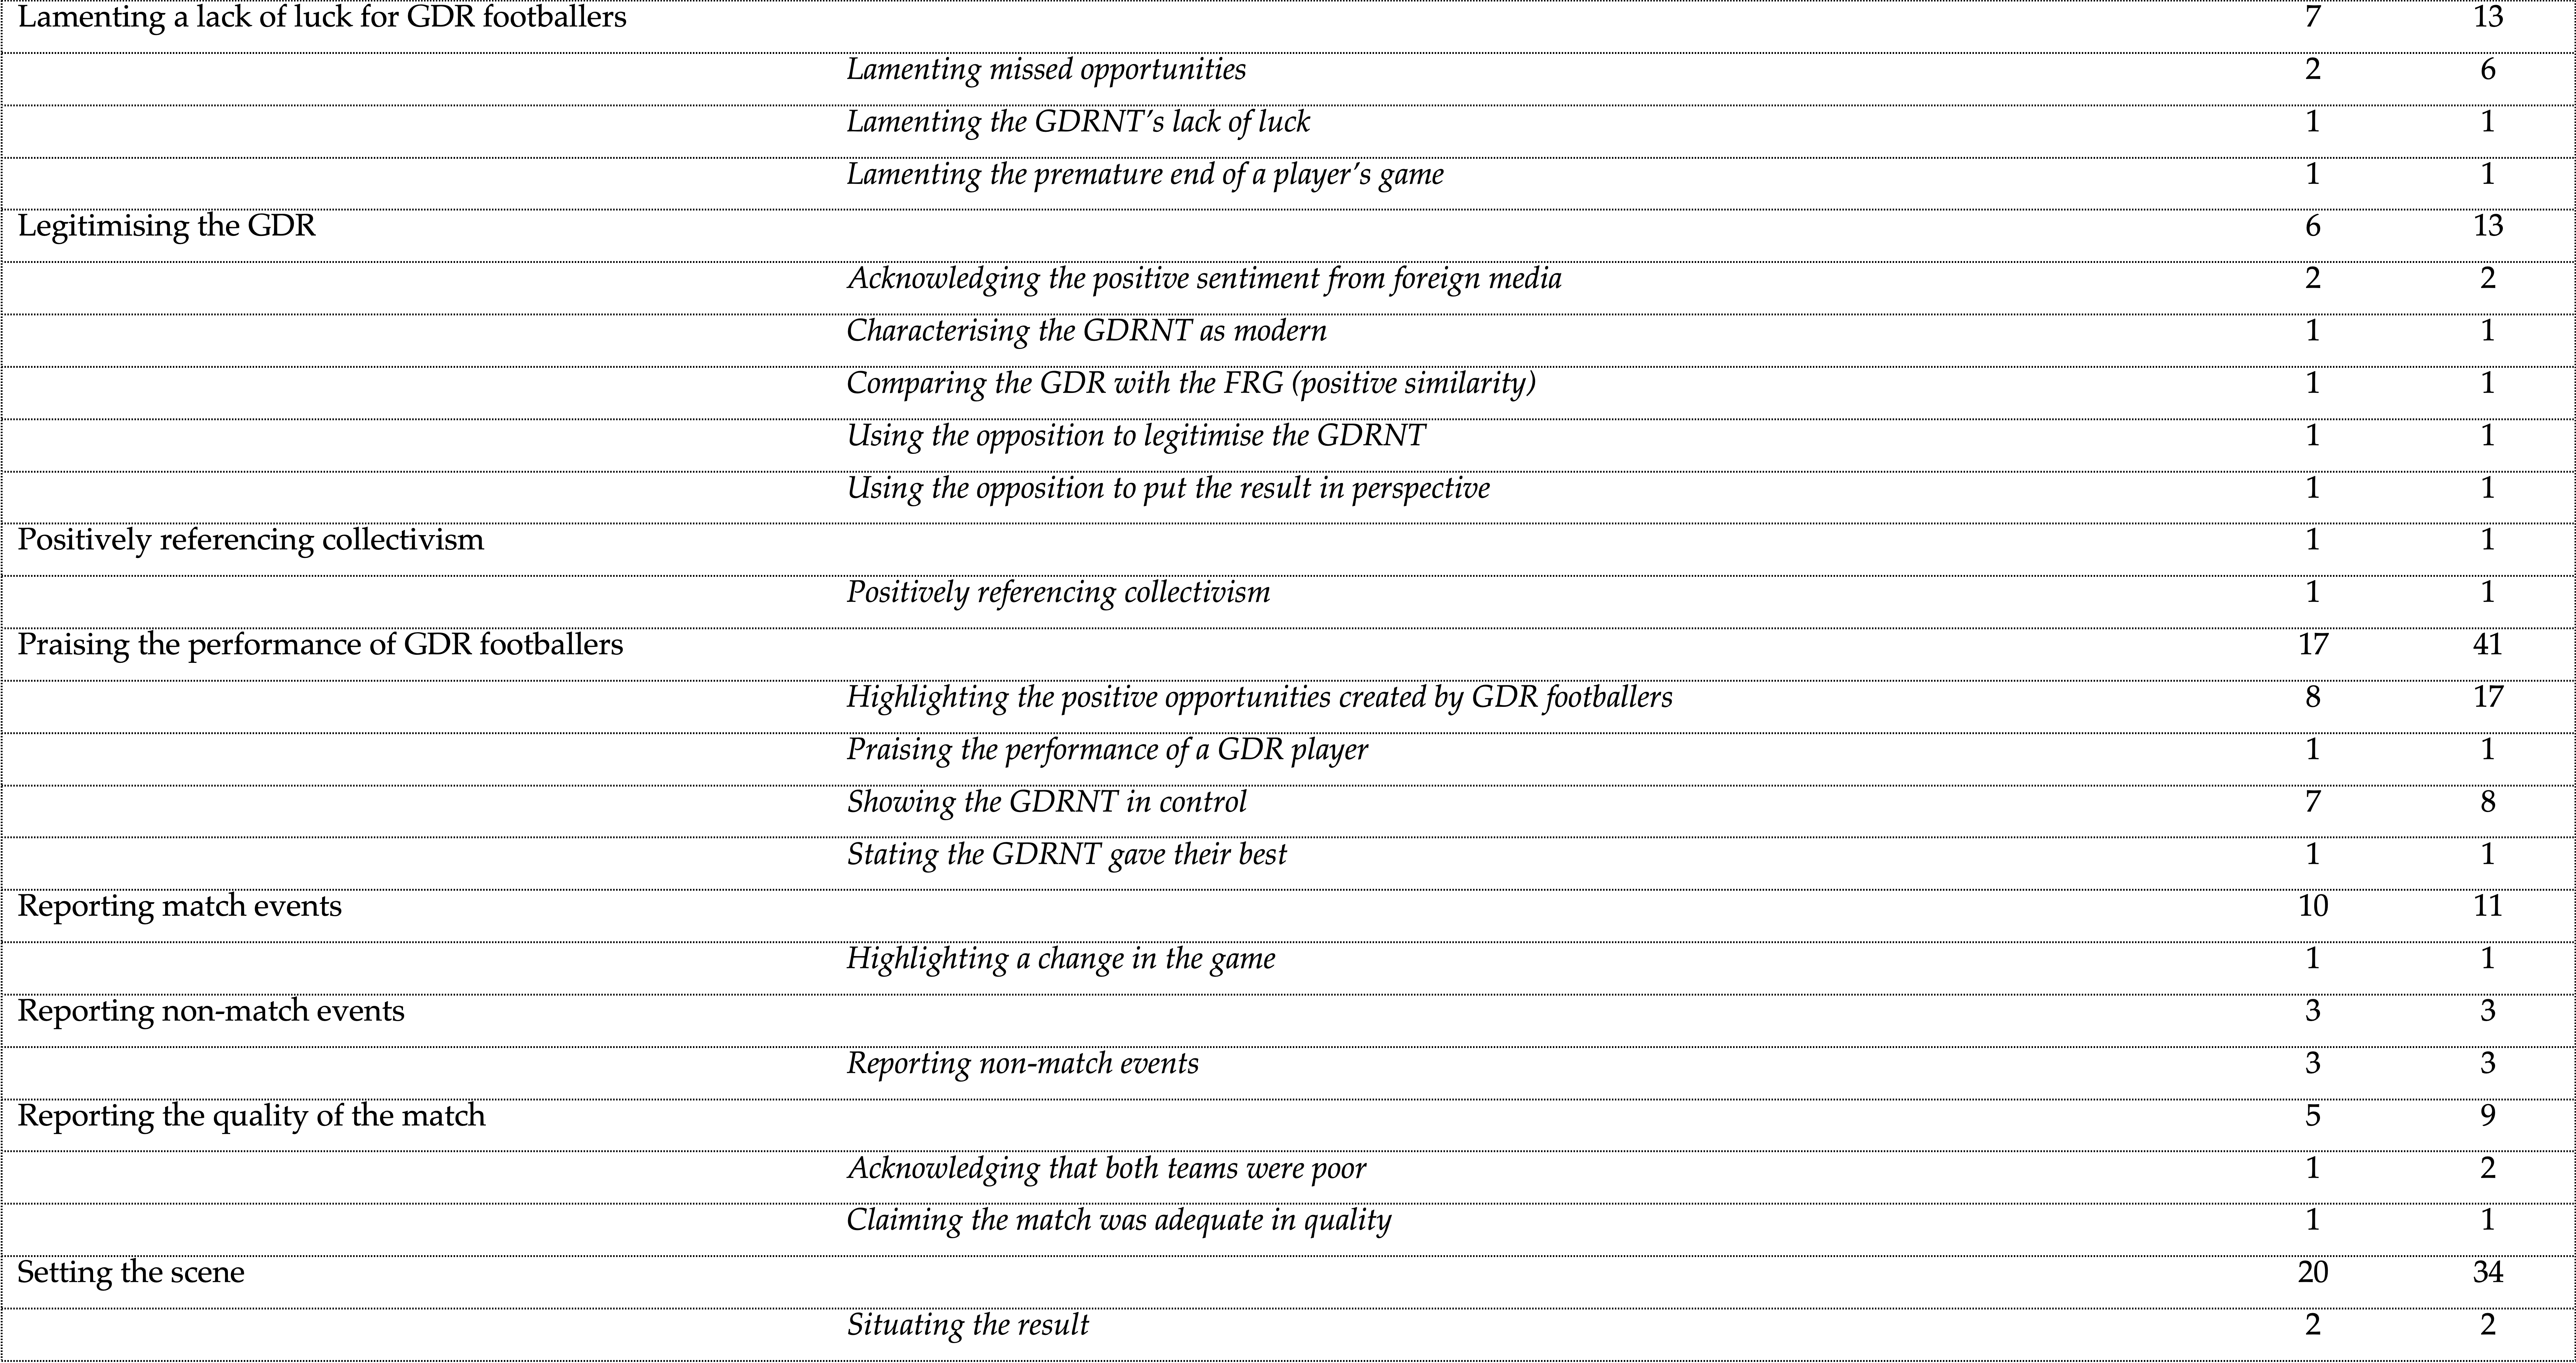
\includegraphics[width=\linewidth]{mres/images/appendix/a5.png}
\end{figure}
\end{landscape}

\begin{landscape}
\begin{figure}[h]
\centering
\bigskip\bigskip\bigskip\bigskip\bigskip
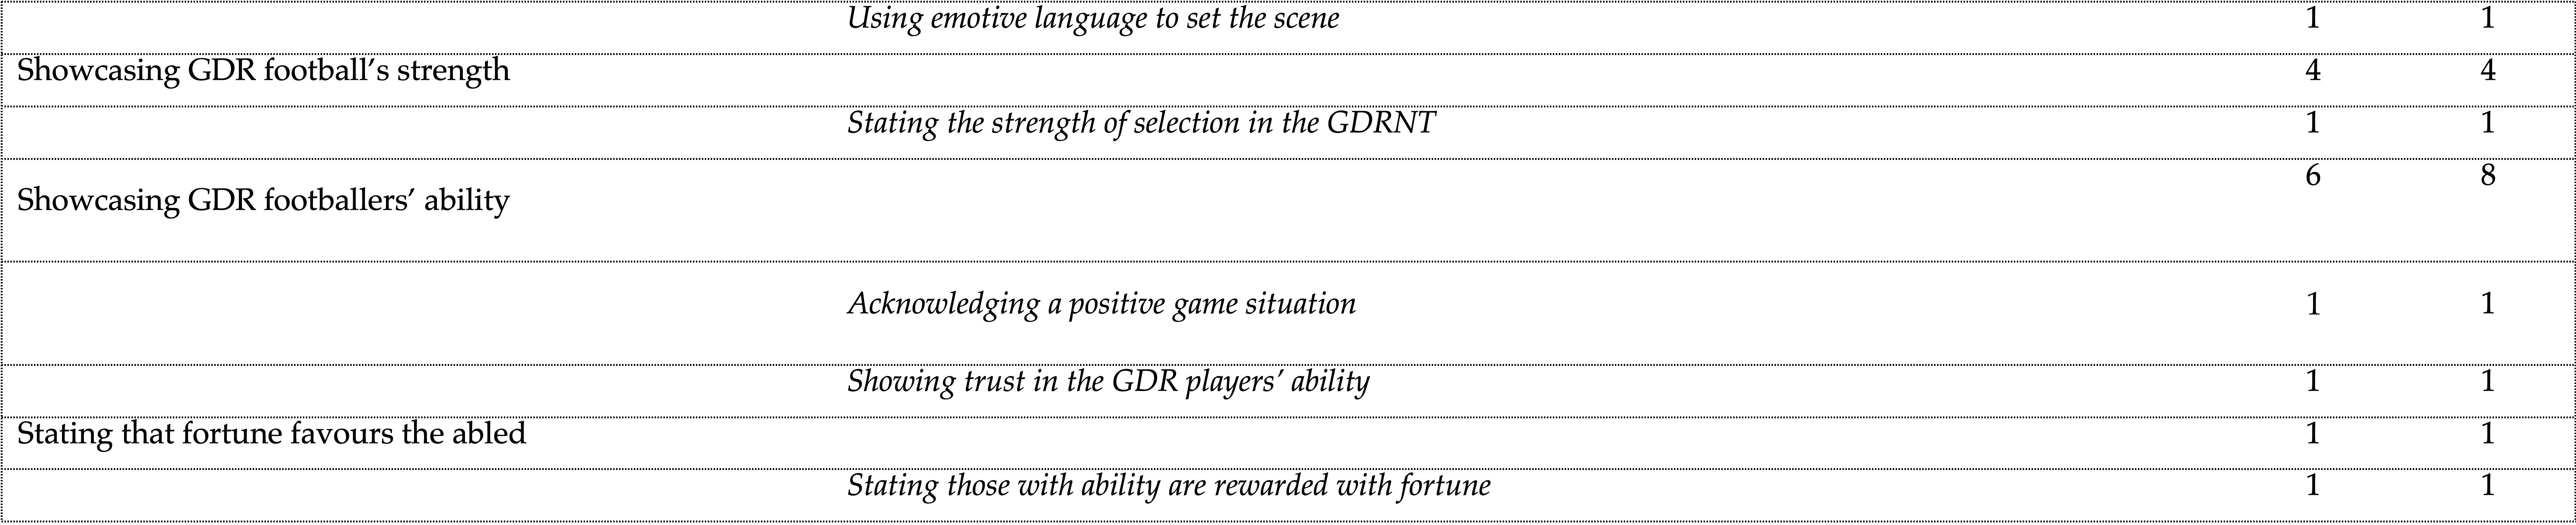
\includegraphics[width=\linewidth]{mres/images/appendix/a6.png}
\end{figure}
\end{landscape}

\chapter{Example of initial coding}

Appendix B shows the initial line-by-line coding performed on the first article analysed, \textit{Gut gekämpft – Siegestor fiel nicht}. The highlighted yellow text are coded references. The coloured coding stripes in the right window signify which initial code the references relate to. 

\begin{landscape}
\begin{figure}[h]
\centering
\bigskip\bigskip\bigskip
\caption{Screen shot of initial coding for the article \textit{Gut gekämpft - Siegestor fiel nicht} in NVivo 12}
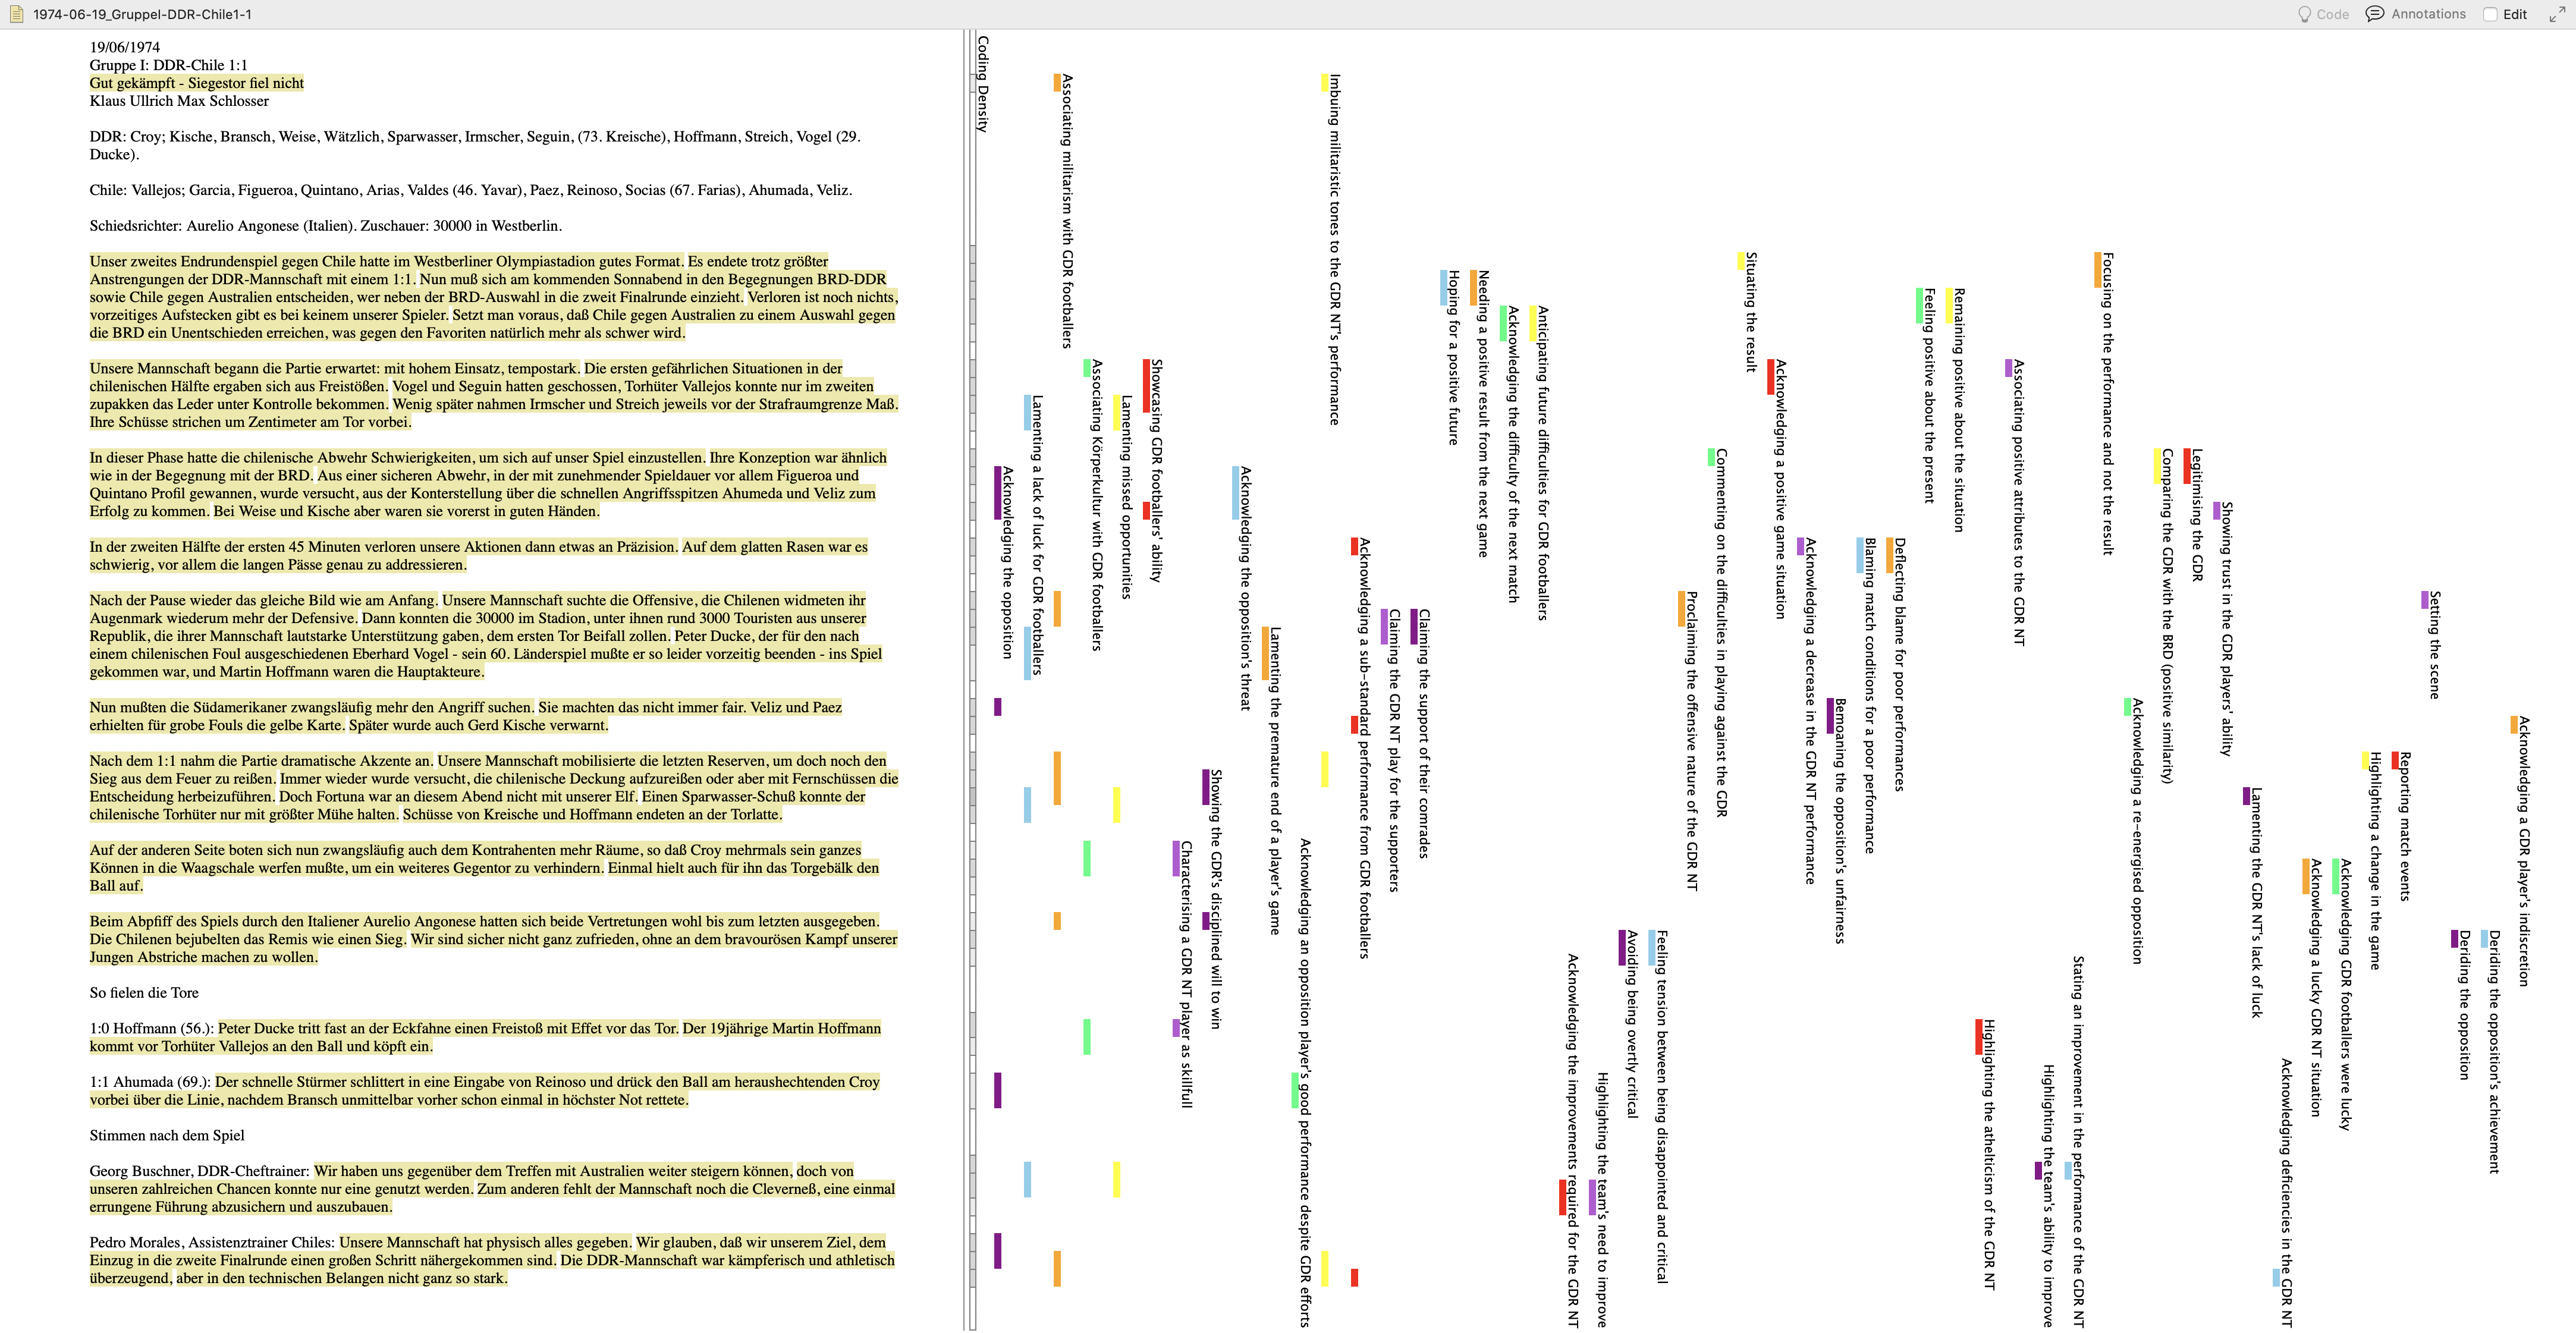
\includegraphics[width=\linewidth]{mres/images/appendix/b1.png}
\end{figure}
\end{landscape}

\chapter{Example of category coding}

Appendix C shows the category coding performed on the sixth article analysed, \textit{Gute Aktionen und ein schönes Tor}. The highlighted yellow text are coded references. The coloured coding stripes in the right window signify which category the references relate to. 

\begin{landscape}
\begin{figure}[h]
\centering
\bigskip\bigskip\bigskip
\caption{Screen shot of category coding for the article \textit{Gute Aktionen und ein schönes Tor in NVivo 12}}
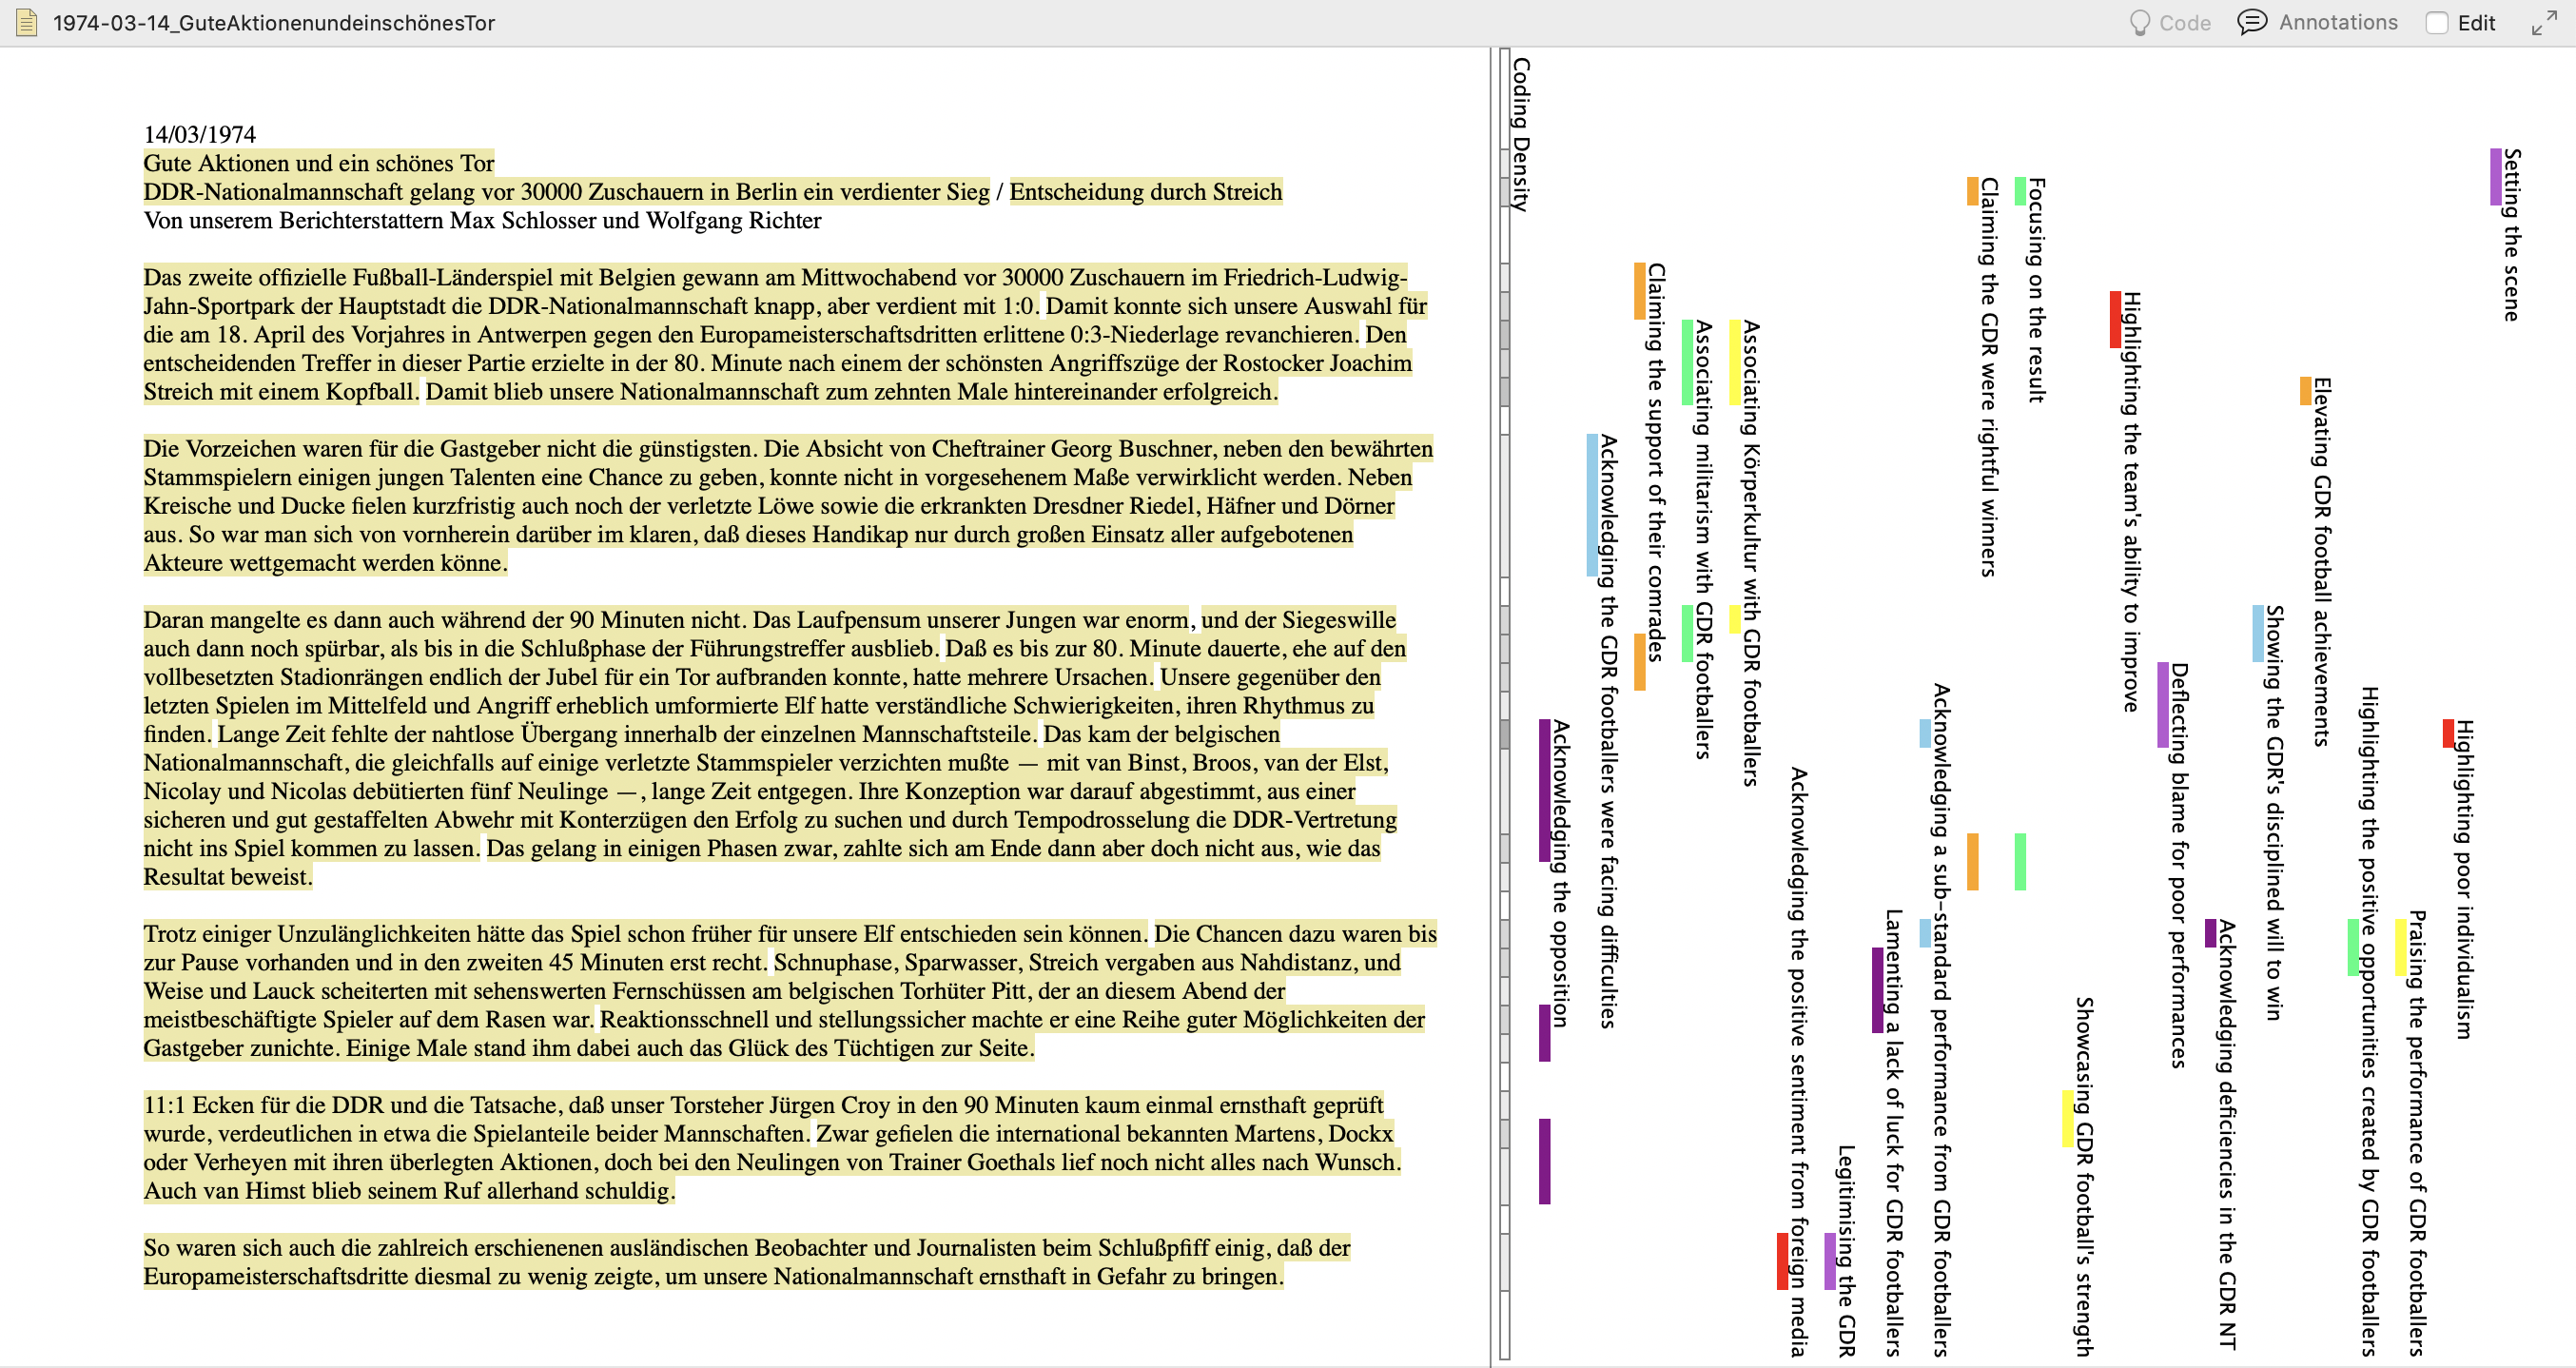
\includegraphics[width=\linewidth]{mres/images/appendix/c1.png}
\end{figure}
\end{landscape}
